
\renewcommand{\thefigure}{\roman{figure}} % See here for other options: http://timmurphy.org/2011/07/18/latex-table-and-figure-numbering-style/
\setcounter{figure}{0}

\chapter*{Future directions}\label{ch:conclusion}
\addcontentsline{toc}{chapter}{Future directions}

% Main points:
% - What has been accomplished that was not there before
% - What is the most relevant follow up work
% - What are the most relevant challenges
% - Make sure to connect with the introduction, that is refer to the problems presented there and the degree to wich they are addressed.


% 1. Accomplishments (Separate technical and scientific?)
% - Use of system level models
% - Develop multi-objective optimzation formualtions and solution techniques, with the primary aim of modular design, but applicable to many design and analysis situtations were multiple conflicting objectives exist -> for example?
% - ...
% - (reference to the arrow figure)


%TODO: Could move the contribution to later in the pargraph?
%In this thesis we have developed quantitative and systematic tools for modular design of cellular systems, primarly through multi-objective optimization theory.
%The driving application behind these developments is
Whole-cell biocatalysis technology can lead to renewable and sustainable manufacturing of chemicals, fuels, and materials.
Over the past two decades, researchers at companies and universities have been developing platform strains that can produce various metabolically similar molecules \citep{nielsen2016}.
However, these efforts have been limited by the use of qualitative and reductionistic approaches.
Motivated by the potential of modular platform strains, we used multi-objective optimization theory and  genome-scale metabolic models to develop several iterations of the ModCell design method (Figure~\ref{fig8:arrow}).
We applied ModCell tools to design \textit{E.~coli} and \textit{C.~thermocellum} modular cells that enable various product synthesis phenotypes in a plug-and-play fashion.
These proposed modular cell designs require few genetic manipulations thanks to the natural modular features of metabolic networks.
Overall, this effort contributes to the current wave in synthetic biology of tackling problems through more quantitative and holistic approaches.
We envision the new design tools will help reduce the cost and time required to develop efficient and robust biocatalytic strains that harness the large space of molecules resulting from natural and synthetic metabolic pathways.

\begin{figure}[h]
  \centering
  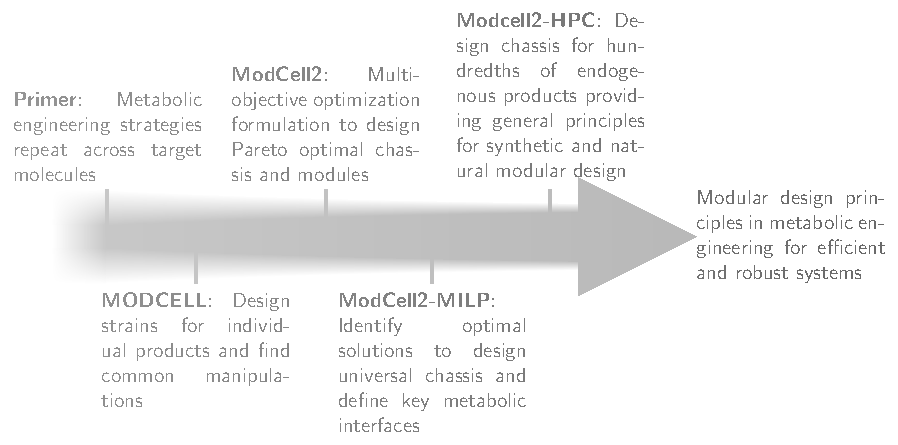
\includegraphics[width=\textwidth]{timeline-arrow}
    \caption[Developments in modular cell design tools]{Developments in modular cell design tools: Primer (Chapter~\ref{ch:review}), MODCELL \citep{trinh2015}, ModCell2 (Chapter~\ref{ch:modcell2}), ModCell-MILP (Chapter~\ref{ch:milp}), ModCell-HPC (Chapter~\ref{ch:hpc}).}
    \label{fig8:arrow}
\end{figure}


% 2. Next wave: The need of the problem framing to build and study strains in this context
% - While techniques have general application,  Predictions without validation is only part of the story.
% - There are two views: 1)design simulation to build; 2)Use simulation to contextualize
% - Modcell falls in case 1. The problem formulation requires that experimental data is ... this was as much as possible done by examining the literature, primarly in the field of metabolic engineering, where genetic manipulations are implemented and characterized ...
% - C therm chapter is case 2.
% - Next wave -> build and characterize

% TODO: The main point does not stand out, and the beginning of the paragraph feels confusing
The interdisciplinary nature of computational biology demands that one addresses algorithmic and modeling challenges, while also combining simulation efforts with experimental validation.
To bridge the gap between simulations and experiments, a simulation can be used to generate a testable hypothesis, or a simulation can be used to explained existing data.
Chapter~\ref{ch:ctherm} is an example of the second case, where proteomics data studied through model simulations increases our understanding of redox metabolism in \textit{C.~thermocellum} biofuel-producing strains.
However, the majority of this work, formulated as a biocatalysis strain design problem, falls under the first case.
Hence, the next wave of development of modular cell design principles should be focused on the implementation and characterization of the strains proposed here, closing the design-build-test-learn cycle.

%post hoc addition of experimental data %Watch out since post hoc, can have quite negative connotations %Watch out since post hoc, can have quite negative connotations


% 3. Future perspective (be general and tie back to the **intro**)
% - Main challenges in the relevant fields
% - highly predictive does not seem around the corner
% - time horizon for application
% - Ethical concerns: Increased inequality and existential risk

As with most contemporary research works, this thesis contributes a drop to the ocean of knowledge needed to address the scientific and social challenges of our time.
%Scientific and social challenges,
The implementation of modular design principles developed here can be impactful in addressing the challenge of whole-cell biocatalysis, however, there are other important facets of this problem.
%There are multiple relevant facets to the problem of whole-cell biocatalysis.
Most notably, the predictive and explanatory capacities of cellular models remain highly limited by a lack of tools to integrate disparate data types and to efficiently measure enzymatic kinetics.
%integration ability to integrate disparate data types and the technical challenges of measuring certain parameters such as the catalytic efficiency of each enzyme.
Furthermore, even if the necessary metabolic fluxes and required enzyme concentrations were known, it remains highly challenging to accomplish appropriate enzyme expression and pathway function \textit{in vivo}.
More generally, we lack precise comprehensive description of already known phenomena (e.g., metabolic reactions), and unknown or poorly explored biophysical phenomena (e.g., macromolecular crowding) are likely to highly influence cellular function.
Hence, it is unlikely that we will develop the capacity to manipulate living organisms for any conceivable biological function in a near future.
The good news is that we are rapidly overcoming the key challenges needed for applied technologies, as evidenced by the many biotechnology companies emerging over the last decade.

As we develop novel technologies, we must also become aware of the ethical and existential risks associated with them.
For example, genetic engineering for enhanced cognitive abilities could likely become an expensive medical treatment that increases the wealth gap in society.
These concerns are specially relevant for the field of synthetic biology, as tools continue to become more widely available hence enabling DIY biohacking \citep{bennett2009}.
These developments could pose an existential risk for our current civilization, given that a highly destructive technology becomes sufficiently easy to use,  and such technology cannot be ``uninvented" or effectively policed.
This challenge can be illustrated through The Urn of Inventions metaphor (Figure~\ref{fig8:vwh}) \citep{bostrom2019}. % NOTE: Follow up this sentence to expl
% NOTE: Make sure this feels "complete" but that further reading is available to expand, do not lean on citations. It has to make sense entirely in this context.
% NOTE: Last sentence needs to be conclusive
Briefly, consider technologies to be balls in an urn, and our current strategy is to draw balls as fast as possible, perhaps to obtain wealth, prestige, and citations.
If there is a ``black ball'' technology, which discovery would cause high damage, alternative research strategies should be considered.
In summary, while issues like climate change already receive considerable attention, we should become more aware of other dangers of technological development and create policies accordingly.

\begin{figure}[h]
  \centering
  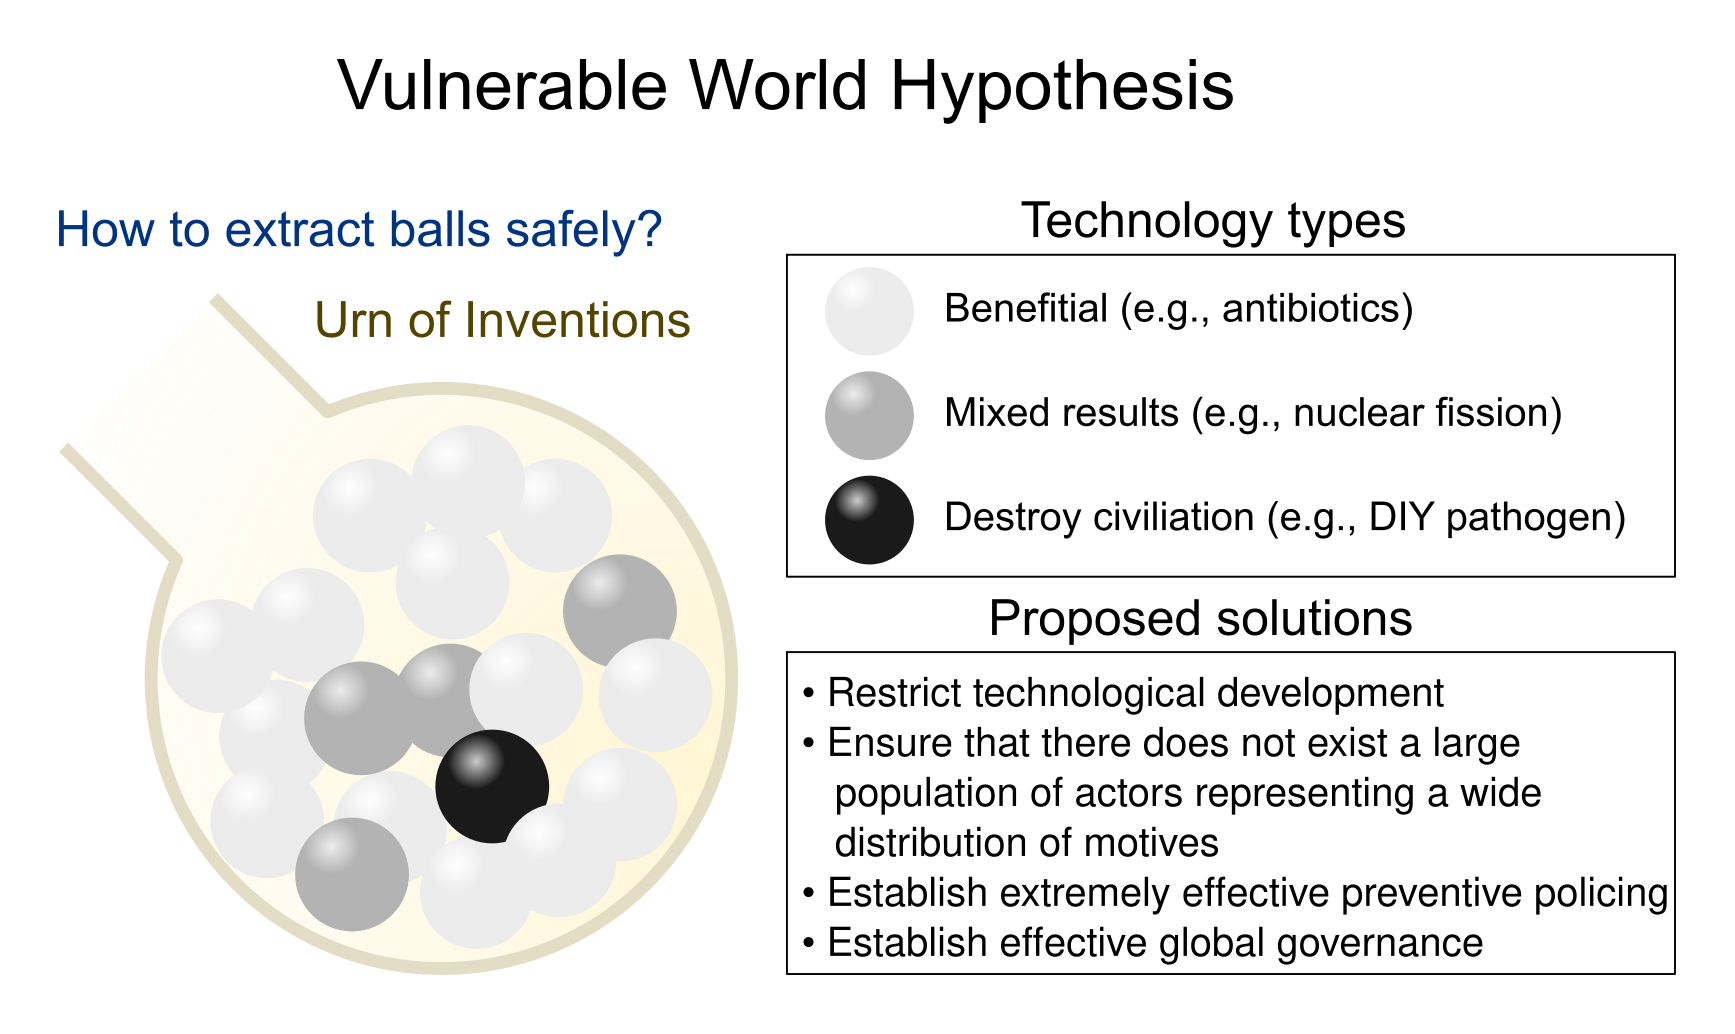
\includegraphics[width=\textwidth]{urn-of-inventions}
    \caption[The Vulnerable World Hypothesis]{The Vulnerable World Hypothesis described through the Urn of Inventions metaphor. The hypothesis is that there exists a technology that once discovered would have devastating effects to civilization. If the hypothesis is true, we should reconsider how scientific and technological discovery is to be conducted to minimize such risk. See \citep{bostrom2019} for further explanation of the topic and proposed solutions.}
    \label{fig8:vwh}
\end{figure}
